\section{Configurazione Collection}
\label{collection}

All'interno della cartella \code{../collection} andranno inseriti i file di configurazione delle Collection. L'applicazione infatti, all'avvio del server, andrà a leggere il contenuto della directory in questione e prelevare sequenzialmente tutti i file con estensione \code{.dsl} contenuti al suo interno. Questi file andranno poi ad essere interpretati dall'interprete DSL, il quale si occuperà di generare tutti i modelli necessari alla configurazione delle varie collection.

La configurazione di una collection avviene tramite l'editing di un file DSL. La configurazione base deve avere la seguente sintassi:
\medskip
\begin{lstlisting}
collection("collectionName","collectionReference", collectionQuery) {
	index {
	}
	show {
	}
}		
\end{lstlisting}

I parametri accettati dalla configurazione di una collection sono i seguenti: 
\begin{itemize}
\item[] \code{\textbf{collectionName}} corrisponde al nome della collection che verrà visualizzato nell'applicazione e deve essere di tipo String;
\item[] \code{\textbf{collectionReference}} corrisponde al nome effettivo della collection nel database MongoDB delle collections e deve essere di tipo String;
\item[] \code{\textbf{collectionQuery}} corrisponde ad un oggetto javascript tramite il quale può essere effettuata una query sulla collection.
\end{itemize}

Ciascuna index-page è composta da una serie di \texttt{column} e può essere configurata come segue: 
\begin{lstlisting}
		index {
			column("columnLabel", "attributeReference", transformation, selectable, sortable)
		}		
\end{lstlisting}
I parametri accettati dalla configurazione di una column di una index-page sono i seguenti: 
\begin{itemize}
\item[] \code{\textbf{columnLabel}} corrisponde al nome visualizzato nell'intestazione della colonna;
\item[] \code{\textbf{attributeReference}} corrisponde al nome effettivo dell'attributo dei document della collection nel database;
\item[] \code{\textbf{transformation}} corrisponde ad una funzione javascript che si occupa di effettuare una trasformazione sul valore dell'attributo. Tale funzione per effettuare l'effettiva trasformazione deve restituire un valore con il \code{return};
\item[] \code{\textbf{selectable}} corrisponde ad un valore booleano che indica se l'elemento della colonna è selezionabile, ovvero se nell'index-page conterrà un link che rimanda alla corrispondente show-page del document;
\item[] \code{\textbf{sortable}} corrisponde ad un valore booleano che indica se la tabella è ordinabile secondo la colonna.
\end{itemize}

Ciascuna show-page è composta da una serie di \texttt{row} che può essere configurata come segue: 
\begin{lstlisting}
		show {
			row("rowLabel", "attributeReference", transformation)
		}		
\end{lstlisting}
I parametri accettati dalla configurazione di una column di una index-page sono i seguenti: 
\begin{itemize}
\item[] \code{\textbf{rowLabel}} corrisponde al nome visualizzato nell'intestazione della riga;
\item[] \code{\textbf{attributeReference}} corrisponde al nome effettivo dell'attributo del document;
\item[] \code{\textbf{transformation}} corrisponde ad una funzione javascript che si occupa di effettuare una trasformazione sul valore dell'attributo. Tale funzione per effettuare l'effettiva trasformazione deve restituire un valore con il \code{return};
\end{itemize}

Di seguito viene fornita un'immagine di esempio in cui viene configurata l'index-page e la show-page relativa ad una collection di \textit{clienti}. Tale configurazione prende tutti i \textit{clienti} di nazionalità italiana.


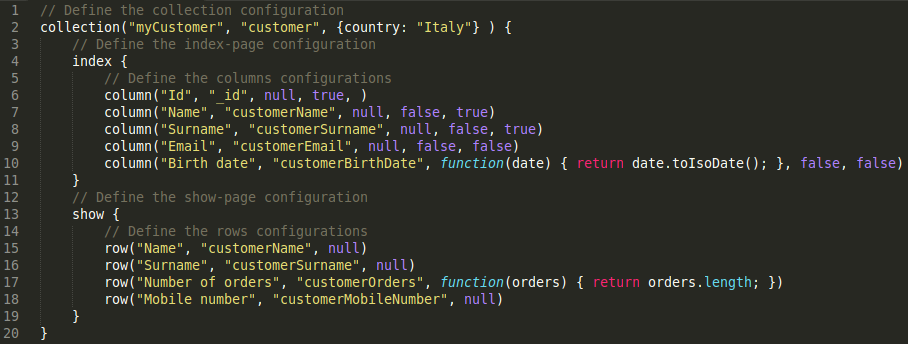
\includegraphics[scale=0.5]{images/dsl-example.png} 